\documentclass[12pt]{article}
\usepackage{graphicx}
\usepackage{amsmath}
\usepackage{mathtools}
\usepackage{gensymb}
\usepackage{tabularx}
\usepackage{array}
\usepackage[latin1]{inputenc}
\usepackage{fullpage}
\usepackage{color}
\usepackage{array}
\usepackage{longtable}
\usepackage{calc}
\usepackage{multirow}
\usepackage{hhline}
\usepackage{ifthen}
\usepackage{lscape}
\usepackage{float}
\usepackage{amssymb}

\newcommand{\mydet}[1]{\ensuremath{\begin{vmatrix}#1\end{vmatrix}}}
\providecommand{\brak}[1]{\ensuremath{\left(#1\right)}}
\providecommand{\norm}[1]{\left\lVert#1\right\rVert}
\providecommand{\abs}[1]{\left\vert#1\right\vert}
\newcommand{\solution}{\noindent \textbf{Solution: }}
\newcommand{\myvec}[1]{\ensuremath{\begin{pmatrix}#1\end{pmatrix}}}
\let\vec\mathbf

\def\inputGnumericTable{}

\begin{document}
\begin{center}
\textbf\large{OPTIMIZATION}

\end{center}
\section*{JEE Maths-65/5/3}

Q26.1 Find the vector equation of the line passing through $\brak{2,1,-1}$ and parallel to the line $\vec{r} = \brak{\hat{i}+\hat{j}}+\lambda\brak{2\hat{i}-\hat{j}+\hat{k}}$. Also, find the distance between these two lines.

\solution
The given equations can be written as
\begin{align}
	\label{eq:eq1}
	\vec{A} &= \vec{x}_1+\lambda_1\vec{m}_1\\
	\label{eq:eq2}
	\vec{B} &= \vec{x}_2 + \lambda_2\vec{m}_2 
\end{align}
where
\begin{align}
	\vec{x}_1 = \myvec{1\\1\\0}, \vec{x}_2 = \myvec{2\\1\\-1},
\end{align}
Also since \eqref{eq:eq1} is parallel to \eqref{eq:eq2} so
\begin{align}
	\vec{m}_1 = \vec{m}_2 = \myvec{2\\-1\\1}
\end{align}
Assume
\begin{align}
	\vec{M} &= \myvec{\vec{m}_1 & \vec{m}_2}\\
	\vec{B}-\vec{A} &= \brak{\lambda_2\vec{m}_2-\lambda_1\vec{m}_1}+\brak{\vec{x}_2-\vec{x}_1}\\
	\label{eq:eq3}
	 &= \vec{M}\vec{\lambda}+\vec{k}\\
	 \text{where } \vec{\lambda}&=\myvec{-\lambda_1\\\lambda_2} \text{ and } \vec{k} = \brak{\vec{x}_2-\vec{x}_1}
\end{align} 
We can formulate an unconstrained optimization problem as below
\begin{align}
	\label{eq:eq4}
	\min_{\lambda} \norm{\vec{B}-\vec{A}}^2
\end{align}
Substituting \eqref{eq:eq3} in \eqref{eq:eq4}
\begin{align}
	\eqref{eq:eq4} &\implies \min_{\lambda}\norm{\vec{M}\vec{\lambda}+\vec{k}}^2\\
	\implies f\brak{\vec{\lambda}} &= \brak{\vec{M}\vec{\lambda}+\vec{k}}^\top\brak{\vec{M}\vec{\lambda}+\vec{k}}\\
	&= \brak{\vec{\lambda}^\top\vec{M}^\top+\vec{k}^\top}\brak{\vec{M}\vec{\lambda}+\vec{k}}\\
	\label{eq:eq5}
	&= \vec{\lambda}^\top\vec{M}^\top\vec{M}\vec{\lambda}+2\vec{k}^\top\vec{M}\vec{\lambda}+\norm{\vec{k}}^2
\end{align}
\eqref{eq:eq5} is a quadratic vector equation. To check whether it is convex or not, we will compute the value of $\vec{M}^\top\vec{M}$.
\begin{align}
	\vec{M}^\top\vec{M} = \myvec{2&-1&1\\2&-1&1}\myvec{2&2\\-1&-1\\1&1} = \myvec{6&6\\6&6}
\end{align}
The eigen values of $\vec{M}^\top\vec{M}$ are 0 and 12, which are greater than equal to zero. Therefore $\vec{M}^\top\vec{M}$ is positive definite matrix implying \eqref{eq:eq5} is convex. Solving the problem in cvxpy yields,
\begin{align}
	\vec{\lambda}_{min} &= \myvec{0.0833\\-0.0833}\\
	\vec{A} &= \myvec{1.167\\0.916\\0.083}\\
	\vec{B} &= \myvec{1.833\\1.083\\-1.083}\\
	\norm{\vec{B}-\vec{A}} &= 1.354
\end{align}
See figure \ref{fig:Fig1}
\begin{figure}[!h]
	\begin{center} 
	    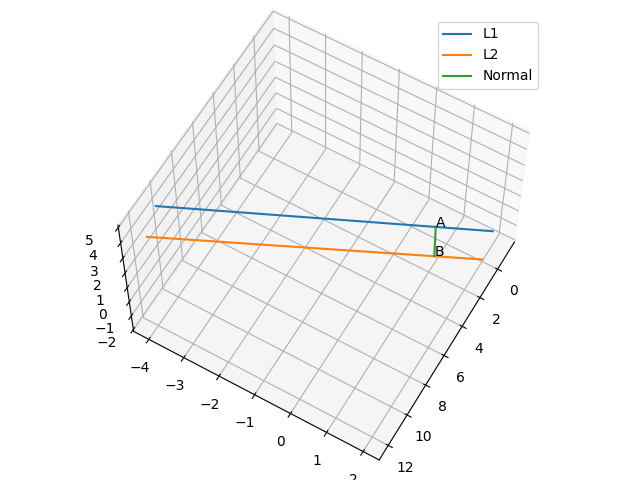
\includegraphics[width=\columnwidth]{figs/jee_q26}
	\end{center}
\caption{}
\label{fig:Fig1}
\end{figure}
\end{document}

























